%%%%%%%%%%%%%%%%%%%%%%%%%%%%%%%%%%%%%%%%%
% University Assignment Title Page 
% LaTeX Template
% Version 1.0 (27/12/12)
%
% This template has been downloaded from:
% http://www.LaTeXTemplates.com
%
% Original author:
% WikiBooks (http://en.wikibooks.org/wiki/LaTeX/Title_Creation)
%
% License:
% CC BY-NC-SA 3.0 (http://creativecommons.org/licenses/by-nc-sa/3.0/)
% 
% Instructions for using this template:
% This title page is capable of being compiled as is. This is not useful for 
% including it in another document. To do this, you have two options: 
%
% 1) Copy/paste everything between \begin{document} and \end{document} 
% starting at \begin{titlepage} and paste this into another LaTeX file where you 
% want your title page.
% OR
% 2) Remove everything outside the \begin{titlepage} and \end{titlepage} and 
% move this file to the same directory as the LaTeX file you wish to add it to. 
% Then add \input{./title_page_1.tex} to your LaTeX file where you want your
% title page.
%
%%%%%%%%%%%%%%%%%%%%%%%%%%%%%%%%%%%%%%%%%
%\title{Title page with logo}
%----------------------------------------------------------------------------------------
%	PACKAGES AND OTHER DOCUMENT CONFIGURATIONS
%----------------------------------------------------------------------------------------
\documentclass[12pt]{article}
\usepackage[spanish, es-tabla]{babel}
\usepackage[utf8x]{inputenc}
\usepackage{amsmath}
\usepackage{graphicx}
\usepackage[colorinlistoftodos]{todonotes}
\usepackage{makeidx}
\usepackage[colorlinks=true,linkcolor=black,anchorcolor=black,citecolor=black,filecolor=black,menucolor=black,runcolor=black,urlcolor=blue]{hyperref}
\usepackage{color}
\usepackage{caption}
\usepackage{etoolbox}
\usepackage{fancybox}
\usepackage{enumitem}
\usepackage{listings}
\lstset{
	language=sh,
	breaklines=true,
	breakatwhitespace=true,
	basicstyle=\ttfamily,
	showstringspaces=false,
	columns=fullflexible-
}
\usepackage{booktabs}
\usepackage{tabularx}
\usepackage{lipsum}
\usepackage{multirow}
\usepackage{caption}
\usepackage{subcaption}

\newcommand\pro{\item[$+$]}
\newcommand\con{\item[$-$]}

\newcommand{\icon}[1]{\includegraphics[height=18pt]{#1}}
\robustify{\icon}
\makeindex
\graphicspath{{./img/}}

\begin{document}

\renewcommand\indexname{Índice}
\begin{titlepage}

\newcommand{\HRule}{\rule{\linewidth}{0.5mm}} % Defines a new command for the horizontal lines, change thickness here

\center % Center everything on the page
 
%----------------------------------------------------------------------------------------
%	HEADING SECTIONS
%----------------------------------------------------------------------------------------

\textsc{\LARGE Facultad de Informática}\\[1.5cm] % Name of your university/college
\textsc{\large Adrián García García}\\[0.5cm] % Minor heading such as course title

%----------------------------------------------------------------------------------------
%	TITLE SECTION
%----------------------------------------------------------------------------------------
\newcommand*{\TitleFont}{%
      \usefont{\encodingdefault}{\rmdefault}{b}{n}%
      \fontsize{19}{23}%
      \selectfont}


\HRule \\[0.4cm]
{ \TitleFont \bfseries Instrumentación del runtime de OpenMP}\\[0.4cm] % Title of your document
\HRule \\[1.5cm]
 
%----------------------------------------------------------------------------------------
%	AUTHOR SECTION
%----------------------------------------------------------------------------------------


% If you don't want a supervisor, uncomment the two lines below and remove the section above
%\Large \emph{Author:}\\
%John \textsc{Smith}\\[3cm] % Your name

%----------------------------------------------------------------------------------------
%	DATE SECTION
%----------------------------------------------------------------------------------------

{\large \today}\\[2cm] % Date, change the \today to a set date if you want to be precise

%----------------------------------------------------------------------------------------
%	LOGO SECTION
%----------------------------------------------------------------------------------------


\includegraphics[width=4cm,keepaspectratio]{logo.png}
 
%----------------------------------------------------------------------------------------

\vfill % Fill the rest of the page with whitespace



\captionsetup[figure]{labelformat=empty,justification=raggedright,singlelinecheck=false}
% Include image from images directory
\begin{figure}[h]

        
\includegraphics[width=2cm,keepaspectratio]{cc-by-sa.png}
        \label{fig:by-sa}
        \caption{ This work is licensed under a \href{https://creativecommons.org/licenses/by/4.0/legalcode}{CC-BY-SA 4.0 License}.}

\end{figure}

\end{titlepage}

\tableofcontents
\clearpage



\section{Introducción}\label{sec:intro}

Este trabajo tiene como objetivo realizar una instrumentación del runtime de OpenMP para permitir la recolección de métricas de rendimiento en los programas que hacen uso de esta API de paralelización. La conferencia relacionada con este trabajo estaba orientada más hacia el paradigma de computación basado en tareas y la paralización de diferentes programas que se ejecutan en procesadores simétricos convencionales. Sin embargo, en el ámbito de investigación en el que participo junto al profesor Juan Carlos Sáez Alcaide hemos observado que la gran mayoría de benchmarks multihilo de suites comerciales (SPEC, PARSEC, Minebench, etc.) hacen uso de directivas de paralelización convencionales como \textit{\#pragma parallel for}. Con el objetivo de evaluar el rendimiento de estos benchmarks, he realizado una instrumentación del runtime de OpenMP y más adelante presentaré un caso de estudio para exponer diferentes retos que debe afrontar su runtime en sistemas multicore asimétricos (AMP).

El modelo de paralelización basado en tareas divide el trabajo en unidades de computación denominadas tareas. El runtime contiene un pool de tareas y un pool de worker threads que ejecutan esas tareas en paralelo. Por otra parte, el modelo de paralelización tradicional de bucles basado en hilos difiere en la forma de gestionar los hilos. En el paradigma basado en tareas, el pool de hilos ejecuta múltiples tareas a lo largo de su tiempo de vida, mientras que en el paradigma de paralelización tradicional los hilos finalizan su ejecución cuando termina la carga de trabajo. Este último modelo se beneficia de la ejecución cargas de trabajo más grandes para evitar la sobrecarga que supone la inicialización de hilos.

La parelización basada en directivas de compilación que reparten el trabajo de los bucles realiza una división del espacio de iteraciones en fragmentos de igual tamaño para cada hilo. No obstante, esta aproximación trae significativos problemas de rendimiento y justicia en los sistemas AMP, ya que sus cores funcionan a diferente frecuencia y pueden presentar características microarquitectónicas diversas (diferentes tamaños de cache, ejecución en orden o fuera de orden, etc.). Estas diferencias provocan que un hilo que se ejecuta en un core big generalmente termine antes su asignación de trabajo. Cuando sucede esto, estos hilos se suelen bloquear en una barrera de memoria a través de una espera activa con el objetivo de sincronizarse con el resto de hilos que se ejecutaban en cores small. Considero que esta situación representa un desperdicio de recursos debido a dos motivos principales:

\begin{itemize}
	\item Los sistemas operativos de propósito general no son capaces de identificar a los hilos que realizan una espera activa y, por tanto, su planificador no puede intercambiar estos hilos por otros que sean capaces de hacer un uso efectivo de los cores.
	\item En el contexto de monitorización del rendimiento y recogida de métricas para la toma de decisiones de planificación, las técnicas de espera activa como mecanismo de sincronización generan unos valores de rendimiento engañosos. Esto se debe a que los hilos que usan estas técnicas producen unos valores altos de IPC, cuando en realidad se encuentran ejecutando instrucciones inútiles para el progreso de la aplicación. Estas medidas pueden llevar a tomar decisiones erróneas al planificador o incluso a realizar cargos adicionales en plataformas de Cloud Computing en las que se factura a los usuarios en base al tiempo de uso de CPU y a diferentes métricas recogidas en tiempo de ejecución.
\end{itemize}


Con el objetivo de recoger información de diferentes métricas de rendimiento he elegido utilizar PMCTrack~\cite{pmctrack}, se trata de una herramienta de monitorización del rendimiento a través de contadores hardware para Linux. Esta herramienta ha sido diseñada especialmente para ayudar a los desarrolladores del kernel en la implementación de algoritmos de planificación que utilicen los datos de los contadores de monitorización del rendimiento (Performance Monitoring Counters - PMCs) para realizar optimizaciones en tiempo de ejecución. A pesar de ser una herramienta orientada al sistema operativo, PMCTrack también está equipada con una serie de componentes en espacio de usuario (bibliotecas, entorno gráfico y de línea de comandos) que permiten obtener información de monitorización de aplicaciones en ejecución. En este trabajo se utilizará la biblioteca de PMCTrack para instrumentar el código del runtime de OpenMP y poder recoger diferentes métricas de los bucles paralelizados con este framework. Se puede encontrar un manual de usuario junto a una guía de instalación en la página web oficial del proyecto~\cite{pmc-userguide}. A continuación se muestra un comando básico cómo ejemplo de uso de PMCTrack, este comando proporciona al usuario el número de instrucciones retiradas y los ciclos de procesador por segundo. Para indicar los conjuntos de eventos hardware a monitorizar, es preciso utilizar la opción -c. Como se muestra en el ejemplo, la herramienta de línea de comandos permite especificar los eventos hardware a monitorizar usando mnemotécnicos. Al final de la línea, se especifica el comando para ejecutar la aplicación que deseamos monitorizar (por ejemplo, ./galgel00).

\begin{lstlisting}[frame=none,language=bash,basicstyle=\tt\scriptsize]
$ pmctrack -c instr,cycles ./galgel00 
[Event-to-counter mappings]
pmc1=instr
pmc2=cycles
[Event counts]
nsample    pid      event          pmc1          pmc2
      1  27204       tick    2247040326    1723742839 
      2  27204       tick    2423705061    1957082929 
      3  27204       tick    2466664612    1944385684 
      4  27204       tick    2280669757    1964700454 
      5  27204       tick    2595158266    1983839065 
      6  27204       tick    2462262543    1980869030 
      7  27204       tick    2474564037    1942807991 
      ...
\end{lstlisting}

\begin{figure}[tbp]
    \centering
    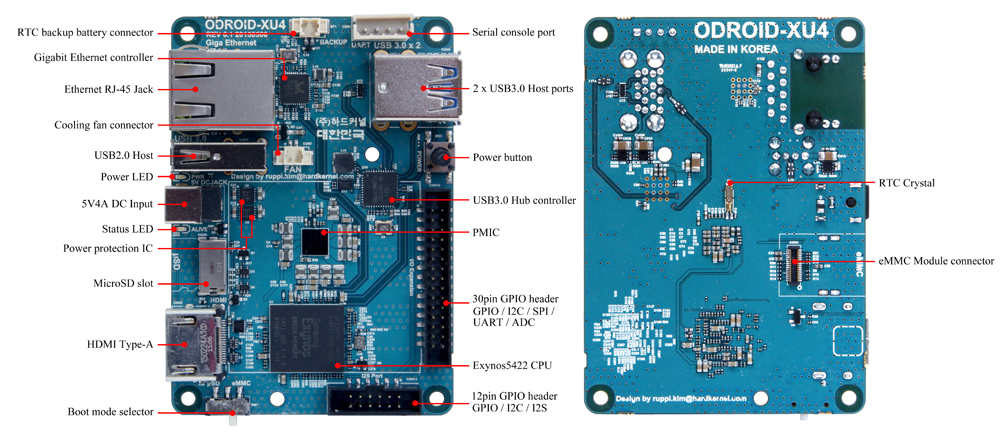
\includegraphics[width=1\textwidth]{foto_placa_XU4.png}
    \caption{Placa ODROID-XU4}
    \label{fig:fotoPlacaXU4}
\end{figure}

Para la realización de este trabajo se ha empleado la placa de desarrollo Odroid XU4~\cite{odroid-manual}, el principal motivo de su elección es que incorpora un procesador multicore asimétrico y, además, ya contaba con experiencia trabajando con ella en el Trabajo de Fin de Grado y anteriores investigaciones. Esta placa está provista de un SoC(\emph{System-On-Chip}) Exynos 5422 de Samsung fabricado en 28nm, que integra un procesador ARM big.LITTLE de ocho núcleos. Estos se dividen en dos clusters, cuatro cores Cortex A15 (2GHz) con ejecución fuera de orden y 2MB de último nivel de cache (L2) y otros cuatro cores Cortex A7 (1.4GHz) con ejecución en orden y 512KB de LLC (L2). Ambos comparten espacio de direcciones para acceder a una memoria principal DDR3 de 2GB que funciona a 750  MHz. Para mostrar la configuración de la placa con mayor detalle, la figura \ref{fig:diagramaDeBloquesXU4} muestra el diagrama de bloques de la placa Odroid XU4.


\begin{figure}[tbp]
    \centering
    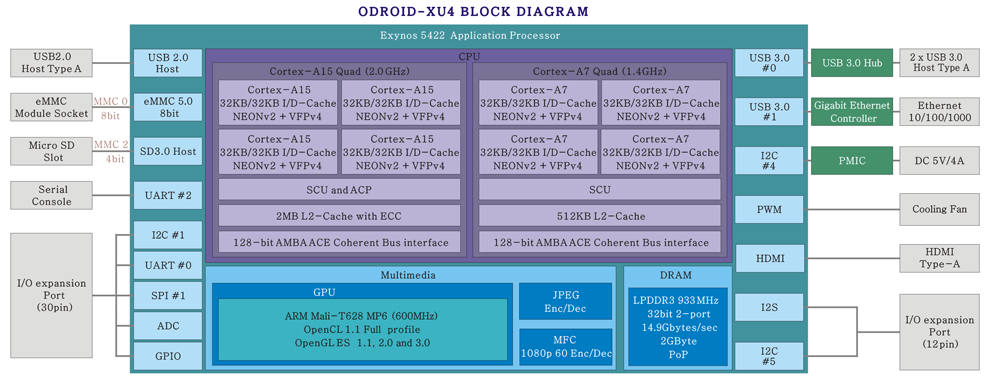
\includegraphics[width=1\textwidth]{diagrama_de_bloques_ODROID_XU4.png}
    \caption{Diagrama de bloques de la placa Odroid XU4}
    \label{fig:diagramaDeBloquesXU4}
\end{figure}


El resto del trabajo está estructurado de la siguiente forma, en la Sección~\ref{sec:expent} se describe de forma detallada el entorno experimental y los pasos seguidos para su construcción. En primer lugar, se explica cómo usar un compilador cruzado y por qué es necesario en la Sección \ref{sec:crucomp}. A continuación, en la Sección~\ref{sec:instrum} se describe el proceso seguido para instrumentar el runtime de OpenMP y en qué partes del código fue necesario introducir llamadas a la librería de PMCTrack para recoger métricas de la paralelización de bucles en tiempo de ejecución. Más adelante, en la Sección~\ref{sec:recolecc} se expone la forma de activar la instrumentación para ejecutar un benchmark y medir el rendimiento de su ejecución con diferentes métricas. Por último, en la Sección~\ref{sec:results} se presentan los resultados obtenidos al instrumentar la ejecución de benchmarks paralelos en la placa Odroid XU4 y en la Sección~\ref{sec:conclu} se exponen las conclusiones que he obtenido durante la realización de este trabajo.

\section{Entorno experimental}\label{sec:expent}

En esta sección expondré los pasos seguidos para construir el entorno experimental usado en este trabajo. Además, introduciré diferentes conceptos relacionados con el runtime de OpenMP. Una buena parte de la información sobre el funcionamiento del runtime y de cómo se puede instrumentar proviene de un Trabajo de Fin de Master de la Universidad de Aalto (Finlandia), llamado "Instrumentation of OpenMP task scheduling" de Marko Rasa~\cite{instrum-omp}. Este trabajo me resultó muy útil como investigación previa para ampliar mis conocimientos sobre OpenMP y su funcionamiento a bajo nivel. Mantiene una aproximación similar, aunque intenta instrumentar la ejecución de programas paralelizados con tareas lo que no representa exactamente el objetivo de este trabajo.

El runtime system de OpenMP provee a los programas de usuario las herramientas para paralelizar su ejecución actuando de interfaz entre el compilador y el sistema operativo, este último expone diferentes recursos como la gestión de memoria dinámica e hilos al runtime. Que a su vez se encarga de proveer una abstracción de estos recursos para que el compilador pueda generar los binarios de diferentes programas, que usan estos recursos mediante llamadas a la librería del runtime system. En la Figura~\ref{fig:compil} se muestran dos esquema, a la derecha se explica la arquitectura explicada anteriormente y a la izquierda se muestra un esquema del proceso de compilación típico de un programa paralelo. Como se explica en \cite{compproc}, el proceso comienza con el código fuente anotado con directivas de compilación. Estas anotaciones son expandidas a llamadas al runtime y tras pasar una fase de optimización el backend del compilador genera el ejecutable final. 

\begin{figure}[tbp]
    \centering
    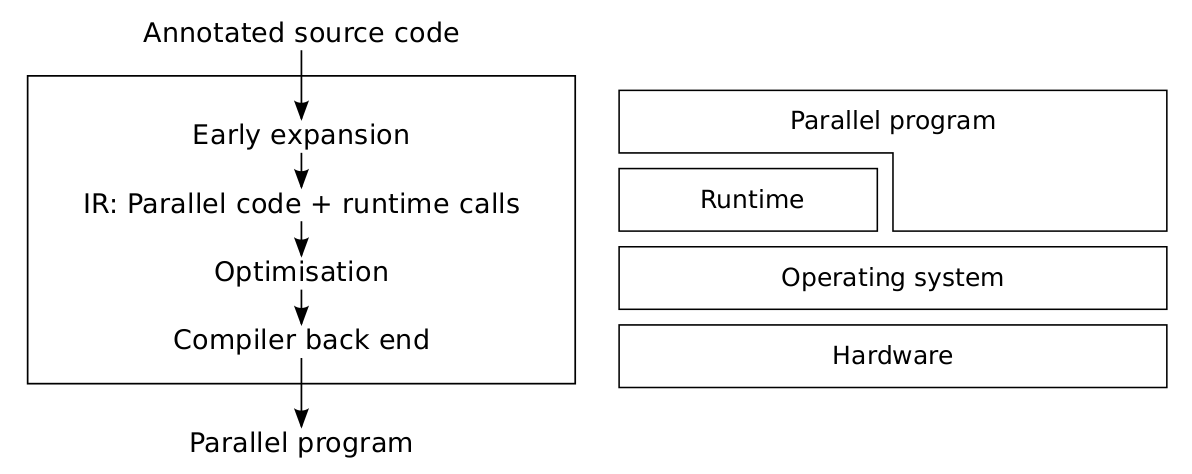
\includegraphics[width=1\textwidth]{scheme.png}
    \caption{Proceso de compilación para un programa paralelo (izquierda) y software stack de la plataforma (derecha).}
    \label{fig:compil}
\end{figure}

El primer problema que debía afrontar era ser capaz de modificar y compilar GCC junto al runtime de OpenMP con el código necesario para instrumentar su ejecución para la arquitectura de 32 bits de ARM de la placa Odroid. Sin embargo, las placas de este tipo tienen una memoria insuficiente para hacer una compilación de GCC junto a sus librerías adicionales, entre ellas la que necesitamos modificar (libgomp). A continuación explicaré el procedimiento seguido.


\subsection{Construcción de un compilador cruzado}\label{sec:crucomp}

El proceso de compilación parte de una máquina de 64 bits con un compilador GCC instalado, que usaremos para construir un compilador cruzado a partir de las fuentes modificadas de libgomp y GCC. La guía seguida para construir un compilador cruzado se puede encontrar en~\cite{crucomp}. Explicaré a grande rasgos los pasos seguidos para su construcción:

\begin{itemize}
  \item En primer lugar se deben generar los compiladores GCC y G++ para la arquitectura x86.
  \item Tras esto, se usarán estos compiladores para generar los headers de la librería estándar de C y los archivos de inicialización (stdio.h, stdlib.h, pthread.h, libc.so, etc.).
  \item Usando los componentes ya generados de Glibc, se continuará con la compilación de la librería de soporte al compilador (libgcc.a y libgcc.so).
  \item En este punto, ya es posible compilar la librería estándar de C (libc.a y libc.so).
  \item Finalmente, compilaremos la librería estándar de C++ (libstdc++.a y libstdc++.so).
\end{itemize}

Una vez completados estos pasos, podremos usar nuestro compilador específico para la arquitectura de 32 bits de ARM para generar los binarios modificados de la librería de OpenMP junto a su runtime system (libgomp).

Durante todo este proceso utilicé la máquina etna07 cómo host para realizar los diferentes pasos del proceso, para hacerlo más sencillo utilicé un túnel SSH y la herramienta sshfs para montar un sistema de ficheros en mi propia máquina que reflejase los cambios al código directamente en etna07 y poder compilar los ficheros allí usando sus 32 cores.

\subsection{Instrumentación del runtime de OpenMP}\label{sec:instrum}

A continuación se explicará el procedimiento seguido para instrumentar el runtime de OpenMP usando la librería de PMCTrack. Con el fin de aprender a usar esta librería, se consultaron los ejemplos disponibles de forma pública junto a las fuentes del proyecto en el repositorio oficial de PMCTrack en GitHub~\cite{pmc-git}.

El objetivo de la instrumentación es escribir los valores de diferentes eventos hardware a un fichero que representen la ejecución de los diferentes bucles de un programa paralelizado con OpenMP. Los pasos seguidos para modificar el código del runtime system son los siguientes:

\begin{itemize}
  \item Copiar en el directorio libgomp/ los ficheros necesarios para enlazar con el modulo del kernel de PMCTrack: pmctrack.h, core.c y pmu\_info.c.
  \item Incluir en el fichero libgomp.h y team.c los archivos copiados anteriormente.
  \item Añadir en la estructura gomp\_thread de libgomp.h un descriptor de fichero  para escribir los resultados de la monitorización y un descriptor de PMCTrack usado para interactuar con la librería (configurar, iniciar y parar los contadores hardware).
  \item El archivo team.c se encarga de gestionar las tareas de inicialización y gestión de un equipo de hilos que paralelizan la ejecución de un bucle. Utilicé la función \emph{gomp\_thread\_start} para inicializar el descriptor de PMCTrack y configurar los eventos hardware que se desean monitorizar.
  \item El archivo loop.c contiene el código que comienza la parelización de los bucles. En concreto, usé la función \emph{gomp\_loop\_init} para colocar la llamada a PMCTrack que pone los contadores en marcha.
  \item Por último, usé la función \emph{free\_work\_share} del archivo team.c para colocar la llamada a la función que para los contadores y escribir la información al fichero de log.
\end{itemize}


\subsection{Recolección de métricas}\label{sec:recolecc}

Para activar y configurar la utilización del código que instrumenta la ejecución de programas paralelos se utilizan una serie de variables de entorno:

\begin{itemize}
  \item GCC\_ROOT: Permite especificar el directorio raíz en el que se encuentran los binarios de GCC y libgomp modificados y compilados específicamente para la arquitectura ARM de 32 bits. 
  \item GOMP\_PMCTRACK: Si se encuentra esta variable de entorno, se activa la monitorización de bucles.
  \item GOMP\_PMCTRACK\_EVENTS: Esta variable permite indicar un string que especifique los eventos de contadores hardware a monitorizar, es posible utilizar tanto el código hexadecimal como mnemotécnicos.
  \item GOMP\_PMCTRACK\_FILE: Permite especificar la ruta a un fichero en el que se volcará la información de los contadores hardware.
  \item GOMP\_PMCTRACK\_NR\_LOOPS: Si se define esta variable de entorno se establece un límite en el número de bucles a monitorizar, tras obtener información de los mismos se acabará con la ejecución del programa.
\end{itemize}

Usando las anteriores variables de configuración, se muestra a continuación un comando para monitorizar el número de instrucciones retiradas, ciclos de procesador completados y fallos de caché de último nivel para los bucles de un programa (\emph{./example}) de la siguiente forma:


\begin{lstlisting}[frame=none,language=bash,basicstyle=\tt\scriptsize]
benchlocal@etna07:~/GCC_OMP/test$ GCC_ROOT=~/GCC_OMP/gcc-git/instdir GOMP_PMCTRACK=1 GOMP_PMCTRACK_EVENTS=instr,cycles,llc_misses GOMP_PMCTRACK_FILE=${PWD}/a.txt GOMP_PMCTRACK_NR_LOOPS  OMP_NUM_THREADS=1 ./example
Number of threads = 1
Thread 0: 100000 iterations
Thread 0: 100000 iterations
Thread 0: 100000 iterations

benchlocal@etna07:~/GCC_OMP/test$ cat a.txt
[Event-to-counter mappings]
pmc0=instr
pmc1=cycles
pmc2=llc_misses
[Event counts]
nsample    pid      event          pmc0          pmc1          pmc2
      1  15715       self       2502869       2066839             0
[Event-to-counter mappings]
pmc0=instr
pmc1=cycles
pmc2=llc_misses
[Event counts]
nsample    pid      event          pmc0          pmc1          pmc2
      1  15715       self       2500340       1931197             0
[Event-to-counter mappings]
pmc0=instr
pmc1=cycles
pmc2=llc_misses
[Event counts]
nsample    pid      event          pmc0          pmc1          pmc2
      1  15715       self       2500338       1938776             0
\end{lstlisting}

\section{Resultados}\label{sec:results}

Los experimentos realizados en este trabajo tienen como objetivo motivar la necesidad de que el runtime system de OpenMP sea consciente de las diferencias en rendimiento que los hilos experimentan si paralelizan su ejecución en distintos tipos de cores en un sistema multicore asimétrico. Para ello, se procedió a ejecutar una serie de benchmarks tanto en cores big como small que paralelizan la ejecución de sus bucles con OpenMP mientras se medían diferentes métricas para caracterizar su rendimiento. 

Para parsear los logs de pmctrack y poder generar las gráficas, he creado un script que coge todos los logs de una carpeta filtrando por un array en el que se le puede indicar el número de experimento y utiliza la librería pandas de python junto a matplotlib para crear las diferentes gráficas. Se puede encontrar el script junto a las fuentes de este trabajo en LaTeX en mi repositorio de GitHub~\cite{parsing}.

Para medir el rendimiento he empleado la métrica Speedup Factor o SF, definido como ${MIPS}_{big}/{MIPS}_{small}$, que mide el ratio de rendimiento producido cuando un programa se ejecuta en un core big respecto a uno small. En los siguientes resultados presento dos tipos de gráfica, por una parte una que representa la evolución de los valores de SF medidos a lo largo del tiempo durante la ejecución de los diferentes bucles paralelizados con OpenMP y por otra una que presenta el porcentaje de muestras de SF que se caen en las diferentes particiones del espacio de muestras que se generan al dividirlos en rangos de 0.5.

En las Figuras~\ref{fig:b1}, \ref{fig:b2} y \ref{fig:b3} se puede observar las medidas de Speedup Factor (SF) obtenidas durante la ejecución de 3 benchmarks paralelizados con OpenMP. Se tomaron métricas de la ejecución de 8 benchmarks en total, aunque he incluido las gráficas que representan las clases de comportamiento más dispares observados en todo el conjunto de experimentos. Por una parte existen algunos benchmarks, cómo los observados en las Figuras ~\ref{fig:b1} y \ref{fig:b2}, cuyos valores de SF pueden experimentar una gran variabilidad a lo largo de su ejecución y sus bucles pueden presentar diferencias significativas en el beneficio relativo que obtienen al ejecutarse en un core big respecto a uno little. Además, los valores de SF a lo largo del tiempo de la Figura~\ref{fig:b1} muestran como el comportamiento de los benchmarks atraviesa diferentes fases claramente diferenciadas y mantiene un comportamiento que podría ser predicho si el runtime fuera capaz de darse muestrear los valores de diferentes métricas y ajustar su planificación de forma dinámica en tiempo de ejecución. Por otra parte, existen otros benchmarks con un comportamiento similar al observado en la Figura~\ref{fig:b3}, el 100\% de las muestras obtenidas para el benchmark blackscholes caen en la misma partición (2.5 a 3.0) y como se puede observar en la gráfica de variación a lo largo del tiempo la variabilidad es muy pequeña, presentando unos valores muy próximos a 2.6 durante toda la ejecución. 

\begin{figure}
\centering
\begin{subfigure}{.5\textwidth}
  \centering
  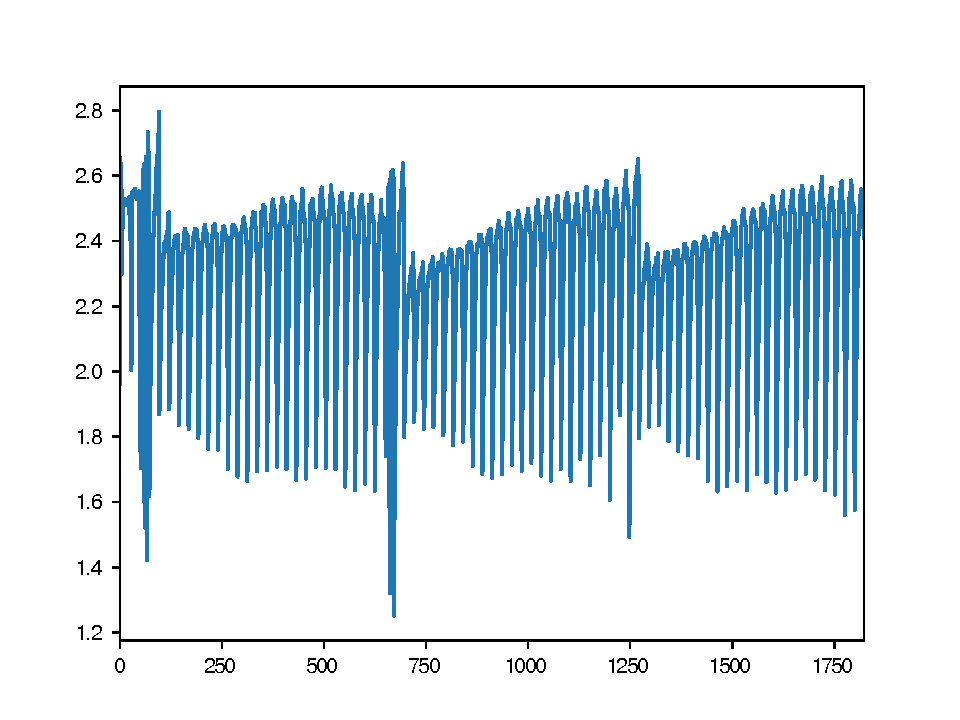
\includegraphics[width=1\linewidth]{sf_over_time_rnaseq.pdf}
\end{subfigure}%
\begin{subfigure}{.5\textwidth}
  \centering
  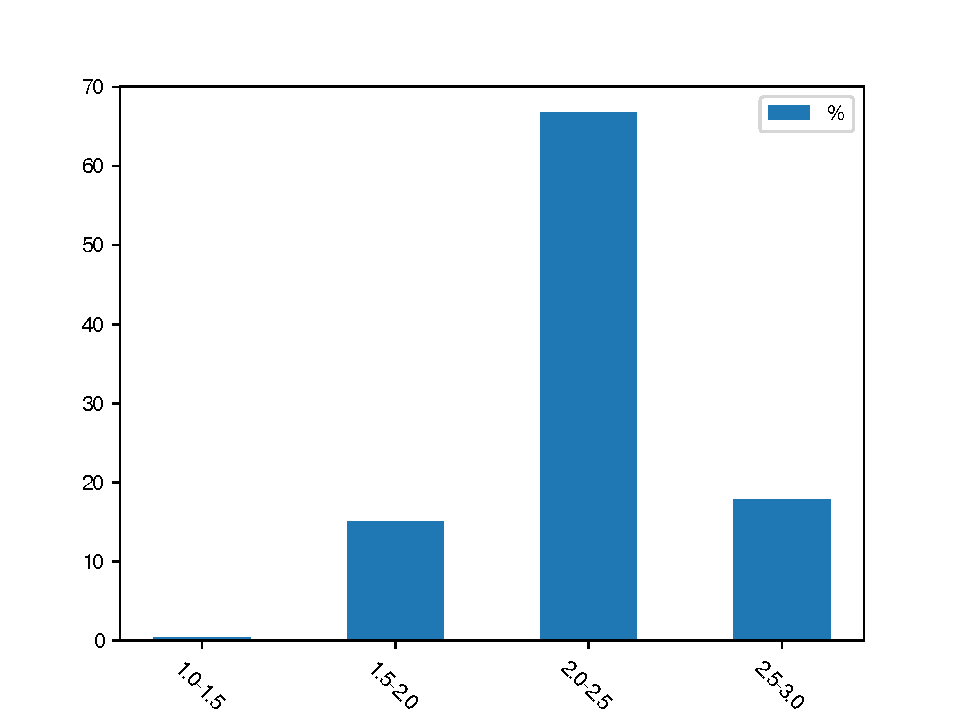
\includegraphics[width=.99\linewidth]{sf_partitions_rnaseq.pdf}
\end{subfigure}
\caption{Variación de SF a lo largo de la ejecución (izda.) y porcentaje de muestras que pertenecen a las diferentes particiones de SF (dcha.) del benchmark rnaseq.}
\label{fig:b1}
\end{figure}

\begin{figure}
\centering
\begin{subfigure}{.5\textwidth}
  \centering
  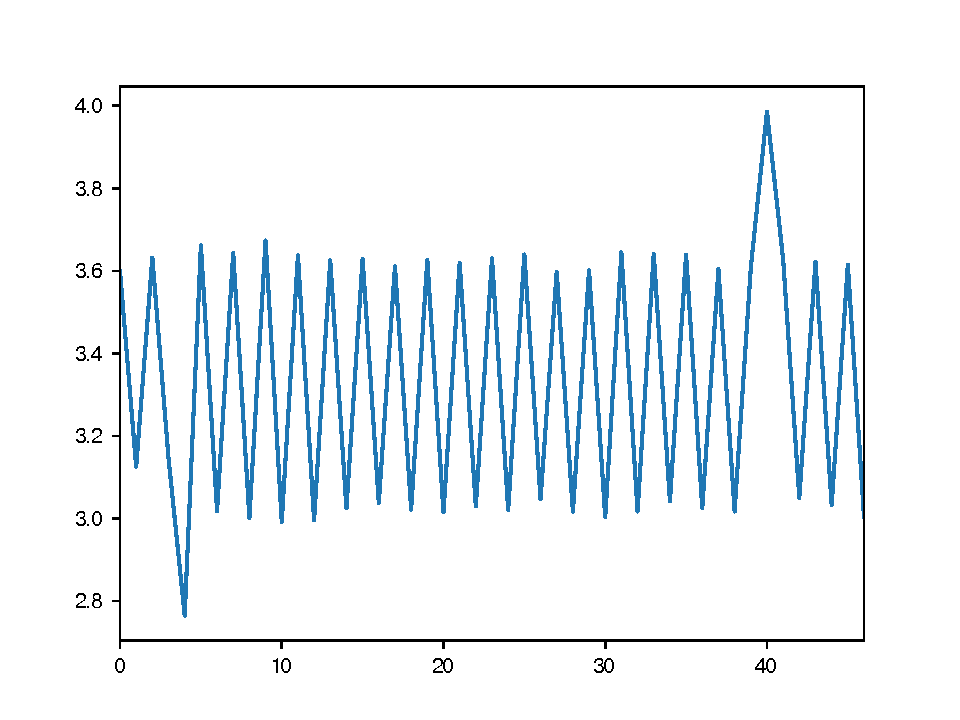
\includegraphics[width=.99\linewidth]{sf_over_time_semphy_mb.pdf}
\end{subfigure}%
\begin{subfigure}{.5\textwidth}
  \centering
  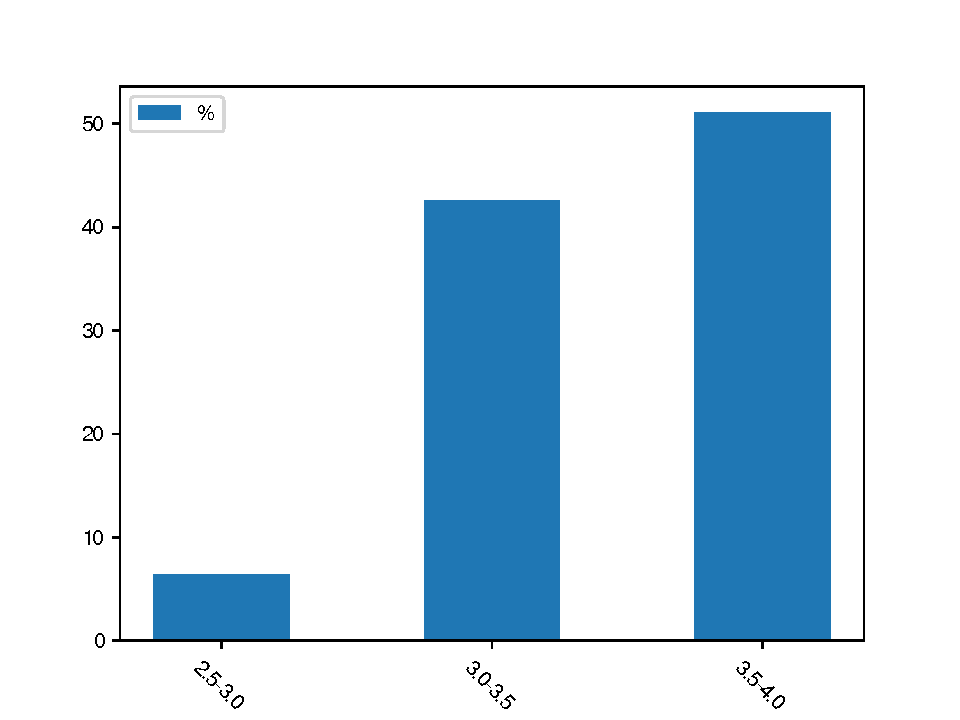
\includegraphics[width=.99\linewidth]{sf_partitions_semphy_mb.pdf}
\end{subfigure}
\caption{Variación de SF a lo largo de la ejecución (izda.) y porcentaje de muestras que pertenecen a las diferentes particiones de SF (dcha.) del benchmark semphy de Minebench.}
\label{fig:b2}
\end{figure}
\begin{figure}
\centering
\begin{subfigure}{.5\textwidth}
  \centering
  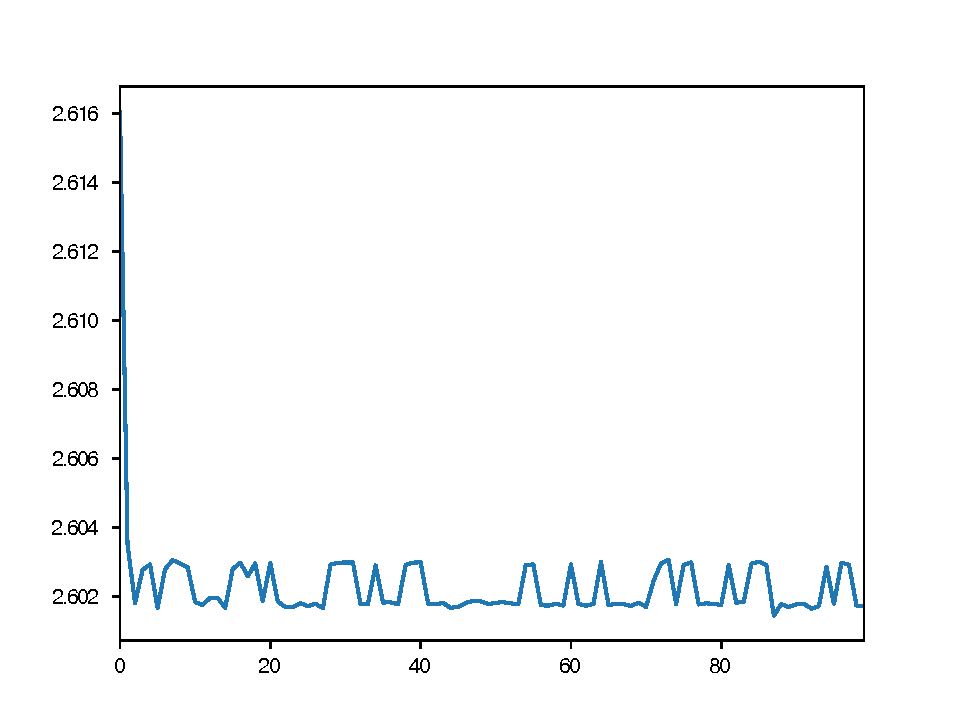
\includegraphics[width=.99\linewidth]{sf_over_time_blackscholes-omp_p.pdf}
\end{subfigure}%
\begin{subfigure}{.5\textwidth}
  \centering
  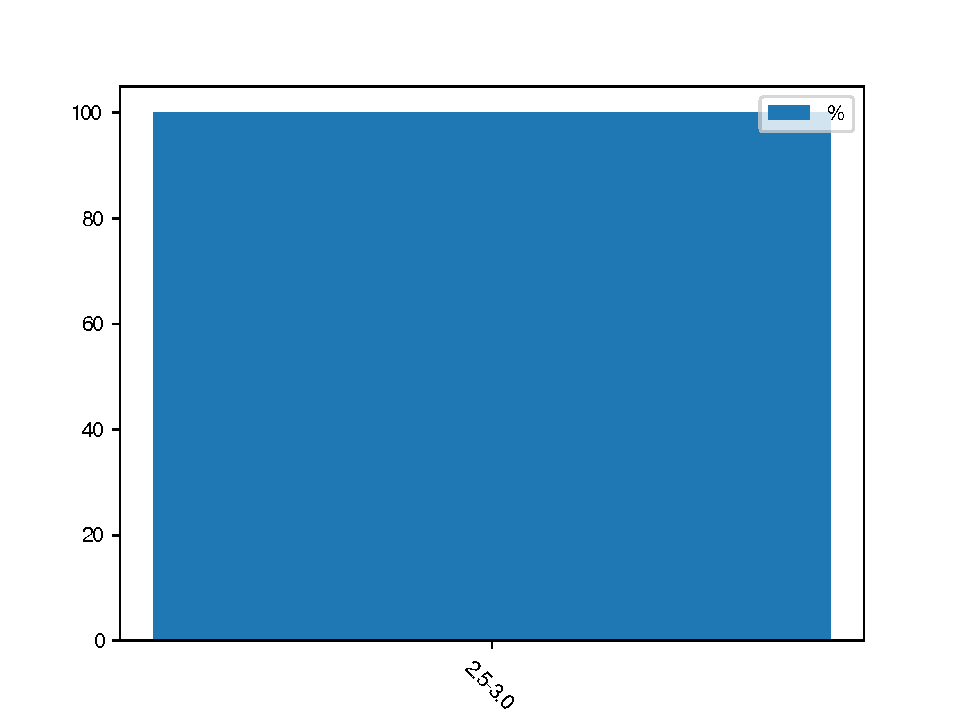
\includegraphics[width=.99\linewidth]{sf_partitions_blackscholes-omp_p.pdf}
\end{subfigure}
\caption{Variación de SF a lo largo de la ejecución (izda.) y porcentaje de muestras que pertenecen a las diferentes particiones de SF (dcha.) del benchmark blackscholes de PARSEC.}
\label{fig:b3}
\end{figure}



\section{Conclusiones}\label{sec:conclu}

En base a los experimentos realizados, se puede observar que el rendimiento obtenido por los programas paralelizados con OpenMP puede variar en gran medida cuando se ejecutan en cores con diferentes características. El hecho de que el runtime system ignore este hecho, genera situaciones de injusticia y problemas de rendimiento en los sistemas multicore asimétricos, especialmente cuando se ejecutan programas paralelizados con el paradigma tradicional de bucles (la mayor parte de benchmarks multihilo intensivos en CPU son así).

Considero que se podría mejorar enormemente el funcionamiento del runtime system de OpenMP si se implementasen estrategias de planificación que tuviesen en cuenta la variabilidad del Speedup Factor de cada hilo a largo de su ejecución y usase esa información para ajustar las decisiones de planificación del runtime. Por ejemplo, para benchmarks que muestran un comportamiento estable sería posible muestrear sus valores de SF durante una fase inicial de su ejecución y usar esos valores para ajustar la cantidad de trabajo que se le asigna a los hilos en función de si se ejecutan en un core big o uno small. De esta forma, el tiempo que tarda en ejecutar su porción de trabajo podría igualarse independientemente del tipo de core en el que se ejecutan. Estas ideas representan una avenida interesante de trabajo futuro, que posiblemente continuaré como parte de mi colaboración con Juan Carlos Saez Alcaide y que podría formar parte de mi Trabajo de Fin de Máster o, en caso de recibir la beca, de mi Tesis Doctoral.



\begin{thebibliography}{1}
%\bibitem{key} description. \href{https://...}{Enlace}
\bibitem{instrum-omp} Instrumentation of OpenMP task scheduling. Author: Marko Rasa. Master's Thesis of the Degree Programme of Computer Science and Engineering on the Aalto University, Finland.
\bibitem{pmctrack}\textit{An OS-oriented performance monitoring tool for multicore systems}. Saez, J. C., Casas, J., Serrano, A., Rodríguez-Rodríguez, R., Castro, F., Chaver, D., \& Prieto-Matias, M. (2015, August). In European Conference on Parallel Processing (pp. 697-709). Springer International Publishing.
\bibitem{pmc-git} \textit{Repositorio oficial de PMCTrack}. Ejemplos de código utilizados disponibles en \textit{pmctrack/test/test\_libpmctrack/}. \href{https://github.com/jcsaezal/pmctrack}{Enlace a git}.
\bibitem{pmc-userguide} \textit{Manual de usuario y guía de instalación}. \href{https://pmctrack.dacya.ucm.es/getting-started/}{Página web oficial}.
\bibitem{odroid-manual} \textit{Odroid XU4: User Manual}. Hardkernel. \href{http://magazine.odroid.com/odroid-xu4/}{Página web}.
\bibitem{compproc}Antoniu Pop and Albert Cohen. Preserving high-level semantics of parallel programming annotations through the compilation flow of optimizing compilers. In Proceedings of the 15th Workshop on compilers for Parallel Computers (CPC’10), Vienna, Austria, July 2010. \href{https://hal.inria.fr/inria-00551518}{URL}.
\bibitem{crucomp}Guía para la construcción de un compilador cruzado. \href{http://preshing.com/20141119/how-to-build-a-gcc-cross-compiler/}{URL}.
\bibitem{parsing}Fuentes de este trabajo junto al script de python creado para parsear los resultados de pmctrack y generar las gráficas presentadas en este trabajo. \href{https://github.com/mizadri/LaTeX/tree/master/openmp-runtime}{Enlace a GitHub}.

\end{thebibliography}

\end{document}